

\chapter{GPIO and Interrupts}

\section{Interrupts}

\todo{GPIO and Interrutps} \underline{\textit{GPIO and Interrutps}} 

\begin{itemize}

\item \textit{In this section I will add the interrupt part concerning the GPIO from my overleaf writing}

\end{itemize}

\section{Peripheral interrupt interaction: EXTI engine}

Before proceeding to programming, we need to understand how GPIO or any peripheral delivers their interrupt to the processor. \\

\underline{\textit{Note}:} this concept of peripheral interrupt processor interaction is \tbi{vendor specific}.\\

We know from chapter arm cortex, that when dealing with interrupts, we have peripheral side in the MCU, and the processor side. Since we are working with interrupts, we need to see how \tbi{GPIO interrupts are passed to NVIC}.\\

To understand this concept, we open the \textit{reference manual} at section 12.2: external interrupt/event controller (EXTI).\\

\newpage
To handle peripheral interrupts, stm has what is called 
\verb|EXTI|, that is external interrupt controller. It's block diagram is shown in \autoref{fig:gpio_interrupts:exti_engine}.

\begin{figure}[h]
\centering
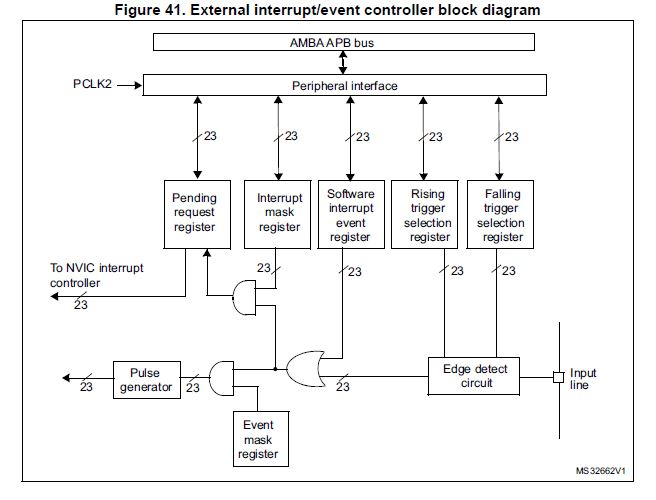
\includegraphics[scale=0.9,frame]{Figures/gpio_interrupts/exti_engine}
\caption{EXTI Peripheral from stm to handle some peripheral interrupts}
\label{fig:gpio_interrupts:exti_engine}
\end{figure}

We can see that this engine is connected to NVIC (which is a peripheral of the processor) using 23 connection. Which means, it captures 23 interrupt positions, or we can say it has 23 different IRQ numbers.

This means if we go to the vector table (table 61 in the reference manual), we should see 23 lines related to EXTI engine.

As example, we can see in IRQ 6 $\rightarrow$ 10, we have EXTI0 till EXTI4.\\

If we go also to IRQ 42, where we have the USB peripheral, we can see that the USB interrupt will go through EXTI, and not directly through NVIC.\\

\newpage
\section{GPIO Interrupts}

As for GPIO, one thing we can notice that if we search the entire table 61 of interrupts, we don't found GPIO peripherals.\\

To understand the GPIO interrupts deliver, we go 12.2.5 in the reference manual, figure 42 (shown in \autoref{fig:gpio_interrupts:exti_gpio})

\begin{figure}[h]
\centering
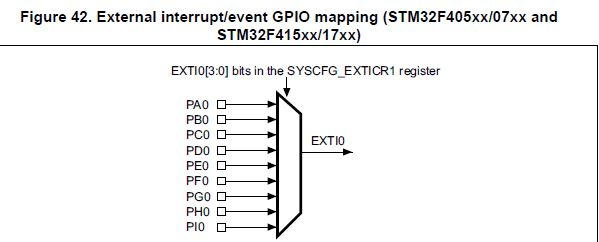
\includegraphics[scale=0.9,frame]{Figures/gpio_interrupts/exti_gpio}
\caption{EXTI engine of stm to handle GPIO interrupts}
\label{fig:gpio_interrupts:exti_gpio}
\end{figure}

    \begin{itemize}
    
    \item We can see that all 0th port ($\mathrm{1}^\mathrm{st}$ pin of each port) of the MCU deliver their interrupt through EXTI0 through a multiplexer, and by configuring  the \verb|SYSCFG_EXTICR1| register.

    \item  We see later that \verb|SYSCFG_EXTICR1| register select the link between a certain port and the EXTI0

        \begin{itemize}
            \item for example, if we connect our button to PD0, we need to configure the link between PD0 line and EXTI0
        \end{itemize}
    
    \end{itemize}

\underline{Summary of Button Interrupt:}

\begin{enumerate}

\item The button is connected to a GPIO pin of the MCU

\item  Configure the GPIO pin to input mode

\item  Link between GPIO pin and EXTI should established through \verb|SYSCFG_EXTICRx| register

\item  Configure the trigger detection (rising, falling or both) for relevant EXTI line

    \begin{itemize}
        \item In \autoref{fig:gpio_interrupts:exti_engine}, we have several register such as Rising trigger selection, falling trigger selection
    \end{itemize}

\item Implement the handler (\verb|C| function) to serve the interrupt

\end{enumerate}

\subsection{EXTI Register}

EXTI register can be found in section 12.3 in the reference manual.

\begin{itemize}

\item \verb|EXTI_IMR| (Interrupt mask register):

    \begin{itemize}
    
        \item Since EXTI desing support for 23 line, only 23 bit of the \verb|EXTI_IMR| can be manipulated

        \item  By default, EXTI doesn't poke the NVIC, we need to enable it through \verb|EXTI_IMR| register, by setting some bit to 1
    
    \end{itemize}

\end{itemize}


All of the above can be summarized in \autoref{fig:gpio_interrupts:gpio_interrupts_block}

\begin{figure}[h]
\centering
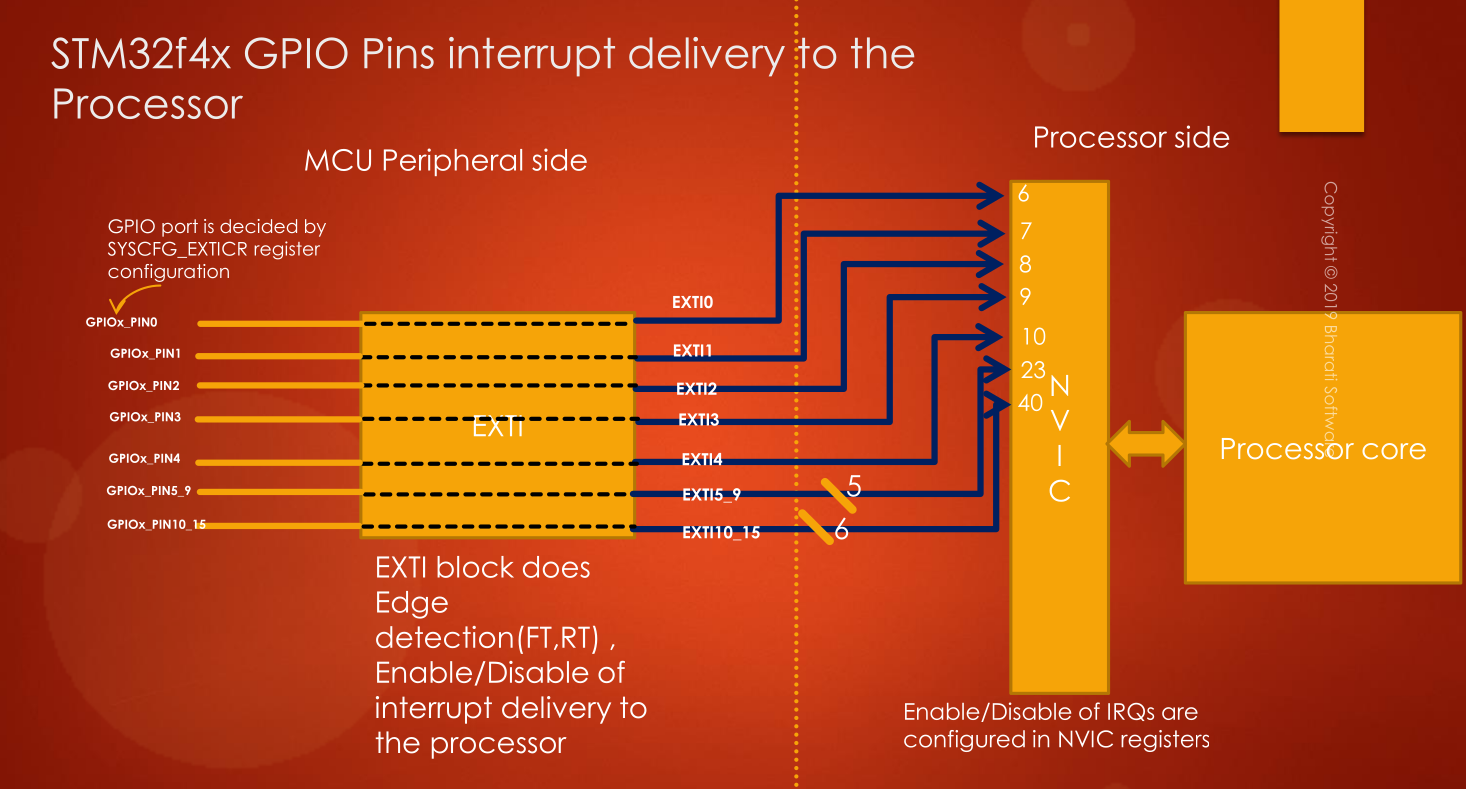
\includegraphics[scale=0.3,frame]{Figures/gpio_interrupts/gpio_interrupts_block}
\caption{GPIO Interrupts flow}
\label{fig:gpio_interrupts:gpio_interrupts_block}
\end{figure}

\begin{itemize}

\item Pin 0 from GPIOx is connected to \verb|EXTI_0|

	\begin{itemize}
	\item This can be viewed also in the reference manual in section 12.2.5, Figure 42
	\end{itemize}

\item The \verb|EXTI_0| engine is connected to \verb|NVIC| (which is again a \textit{processor peripheral}) through IRQ number 6

	\begin{itemize}
	\item The \verb|EXTI_0| connection throuhgh IRQ 6 can be viewed in the vector table, table 62 in section 12.1 in the reference manual
	\end{itemize}

\item Using \verb|NVIC| registers, we could enable or disable the interrupts, becaue by default the interrupts are disabled

\item Remember also that the mapping between pin number from a \verb|GPIOx| and \verb|EXTI| is done via \verb|SYSCFG| (system configuration controller). This is shown also in \autoref{fig:gpio_interrupts:exti_gpio}

	\begin{itemize}
	\item For \verb|SYSCFG|: refer to chapter 9 from the reference manual
	\end{itemize}


\end{itemize}

\newpage
\section{Steps for desiging interrupts}

\begin{enumerate}

\item Pins must be in input mode configuration

	\begin{itemize}
	\item That is because we are receiving interrupts, so we are in input mode
	\end{itemize}

\item Configure the edge detection (rising,falling or both)
	
		\begin{itemize}
		\item That is done through the \verb|EXTI| engine
		\end{itemize}

\item Enable interrupt delivery from peirpheral of the MCU $\rightarrow$ processor


	\begin{itemize}
	\item Done using \verb|EXTI|, so in the MCU side
	\end{itemize}

\item Identiry the IRQ number on which the processor accept the interrupt from that pin

	\begin{itemize}
	\item Done using vector table
	\end{itemize}

\item Configure the IRQ priority for the indentified IRQ number 

	\begin{itemize}
	\item Also done using \verb|NVIC|
	\end{itemize}

\item Enable interrupt reception on that IRQ number 

\item Implement the IRQ handler

\end{enumerate}





